\begin{frame}[fragile]
  \frametitle{Packages required for reproducing the slides}
  
\begin{knitrout}
\definecolor{shadecolor}{rgb}{0.969, 0.969, 0.969}\color{fgcolor}\begin{kframe}
\begin{alltt}
\hlkwd{library}\hlstd{(tidyverse)}  \hlcom{# opinionated collection of packages for data manipulation}
\hlkwd{library}\hlstd{(corrplot)}   \hlcom{# fancy plots of matrices as images}
\hlkwd{library}\hlstd{(GGally)}     \hlcom{# extension to ggplot vizualization system}
\hlkwd{library}\hlstd{(ggfortify)}  \hlcom{# extension to ggplot vizualization system}
\hlkwd{library}\hlstd{(mclust)}     \hlcom{# Gaussian mixture models}
\hlkwd{library}\hlstd{(aricode)}    \hlcom{# fast computation of clustering measures}
\hlkwd{library}\hlstd{(animation)}  \hlcom{# kmeans animation slides}
\hlcom{# color and plots themes}
\hlkwd{library}\hlstd{(RColorBrewer)}
\hlstd{pal} \hlkwb{<-} \hlkwd{brewer.pal}\hlstd{(}\hlnum{10}\hlstd{,} \hlstr{"Set3"}\hlstd{)}
\hlkwd{theme_set}\hlstd{(}\hlkwd{theme_bw}\hlstd{())}
\end{alltt}
\end{kframe}
\end{knitrout}
  
\end{frame}

\begin{frame}[fragile]
  \frametitle{Companion data set}
  \framesubtitle{Morphological Measurements on Leptograpsus Crabs}
  
\begin{block}{Description}
\small The crabs data frame has 200 rows and 8 columns, describing 5 morphological measurements on 50 crabs each of two colour forms and both sexes, of the species \textit{Leptograpsus variegatus} collected at Fremantle, W. Australia.
\end{block}
  
\begin{knitrout}
\definecolor{shadecolor}{rgb}{0.969, 0.969, 0.969}\color{fgcolor}\begin{kframe}
\begin{alltt}
\hlstd{crabs} \hlkwb{<-} \hlstd{MASS}\hlopt{::}\hlstd{crabs} \hlopt \hlkwd{select}\hlstd{(}\hlopt{-}\hlstd{index)} \hlopt
  \hlkwd{rename}\hlstd{(}\hlkwc{sex} \hlstd{= sex,}
         \hlkwc{species}         \hlstd{= sp,}
         \hlkwc{frontal_lob}     \hlstd{= FL,}
         \hlkwc{rear_width}      \hlstd{= RW,}
         \hlkwc{carapace_length} \hlstd{= CL,}
         \hlkwc{carapace_width}  \hlstd{= CW,}
         \hlkwc{body_depth}      \hlstd{= BD)}
\hlstd{crabs} \hlopt \hlkwd{select}\hlstd{(sex, species)} \hlopt \hlkwd{summary}\hlstd{()} \hlopt \hlstd{knitr}\hlopt{::}\hlkwd{kable}\hlstd{(}\hlstr{"latex"}\hlstd{)}
\end{alltt}
\end{kframe}
\begin{tabular}{l|l|l}
\hline
  & sex & species\\
\hline
 & F:100 & B:100\\
\hline
 & M:100 & O:100\\
\hline
\end{tabular}


\end{knitrout}
\end{frame}

\begin{frame}[fragile]
  \frametitle{Companion data set II}
  \framesubtitle{Pairs plot of attributes}

\begin{knitrout}
\definecolor{shadecolor}{rgb}{0.969, 0.969, 0.969}\color{fgcolor}\begin{kframe}
\begin{alltt}
\hlkwd{ggpairs}\hlstd{(crabs,} \hlkwc{columns} \hlstd{=} \hlnum{3}\hlopt{:}\hlnum{7}\hlstd{,} \hlkwd{aes}\hlstd{(}\hlkwc{colour} \hlstd{= species,} \hlkwc{shape} \hlstd{= sex))}
\end{alltt}
\end{kframe}
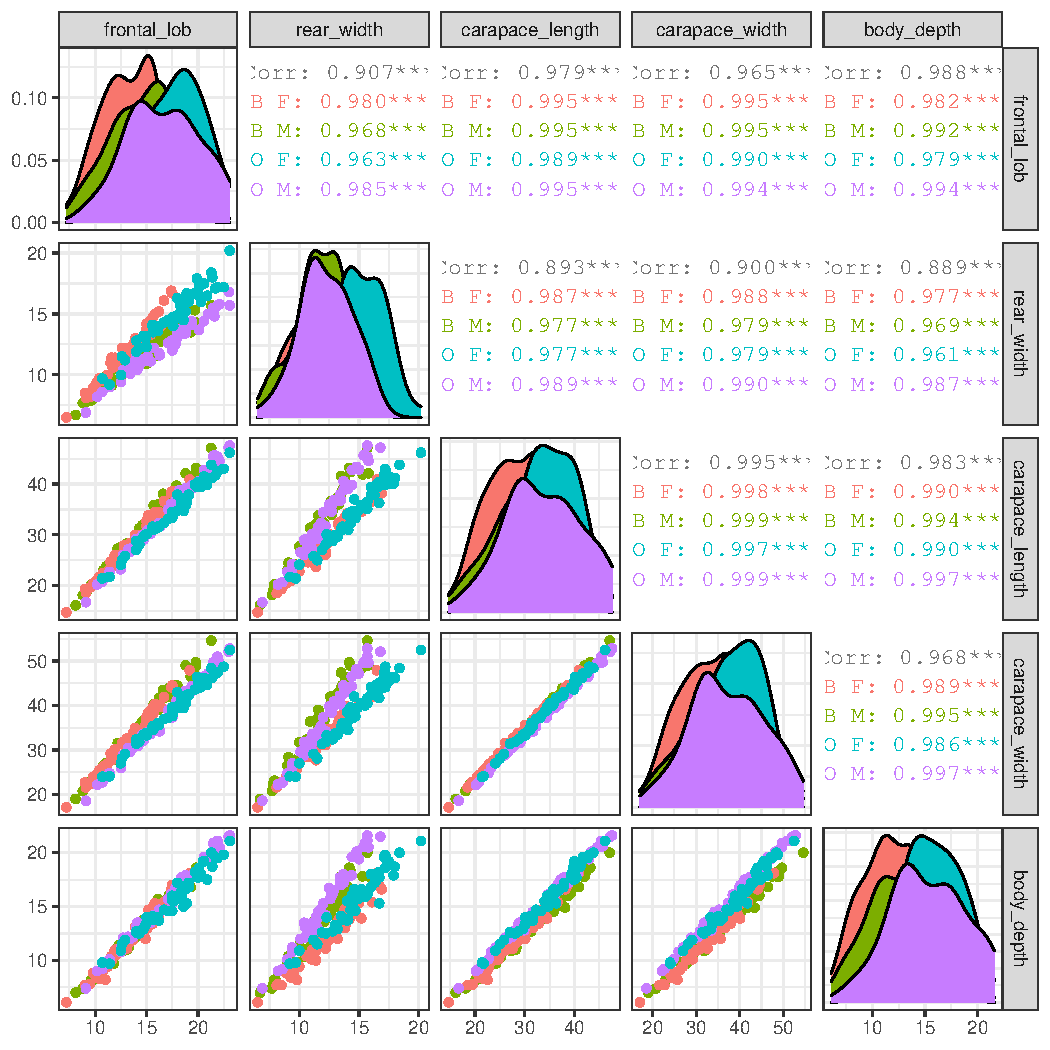
\includegraphics[width=\maxwidth]{figure/crabs_attributes-1} 

\end{knitrout}
\end{frame}

\begin{frame}[fragile]
  \frametitle{Companion data set III}
  \framesubtitle{PCA on the attributes}

\begin{knitrout}
\definecolor{shadecolor}{rgb}{0.969, 0.969, 0.969}\color{fgcolor}\begin{kframe}
\begin{alltt}
\hlkwd{prcomp}\hlstd{(}\hlkwd{select}\hlstd{(crabs,} \hlopt{-}\hlstd{species,} \hlopt{-}\hlstd{sex),} \hlkwc{scale.} \hlstd{=} \hlnum{TRUE}\hlstd{)} \hlopt
  \hlkwd{autoplot}\hlstd{(}\hlkwc{loadings} \hlstd{=} \hlnum{TRUE}\hlstd{,} \hlkwc{loadings.label} \hlstd{=} \hlnum{TRUE}\hlstd{,}
           \hlkwc{data} \hlstd{= crabs,} \hlkwc{colour} \hlstd{=} \hlstr{'species'}\hlstd{,} \hlkwc{shape} \hlstd{=} \hlstr{'sex'}\hlstd{)}
\end{alltt}


{\ttfamily\noindent\color{warningcolor}{\#\# Warning: `select\_()` is deprecated as of dplyr 0.7.0.\\\#\# Please use `select()` instead.\\\#\# This warning is displayed once every 8 hours.\\\#\# Call `lifecycle::last\_warnings()` to see where this warning was generated.}}\end{kframe}
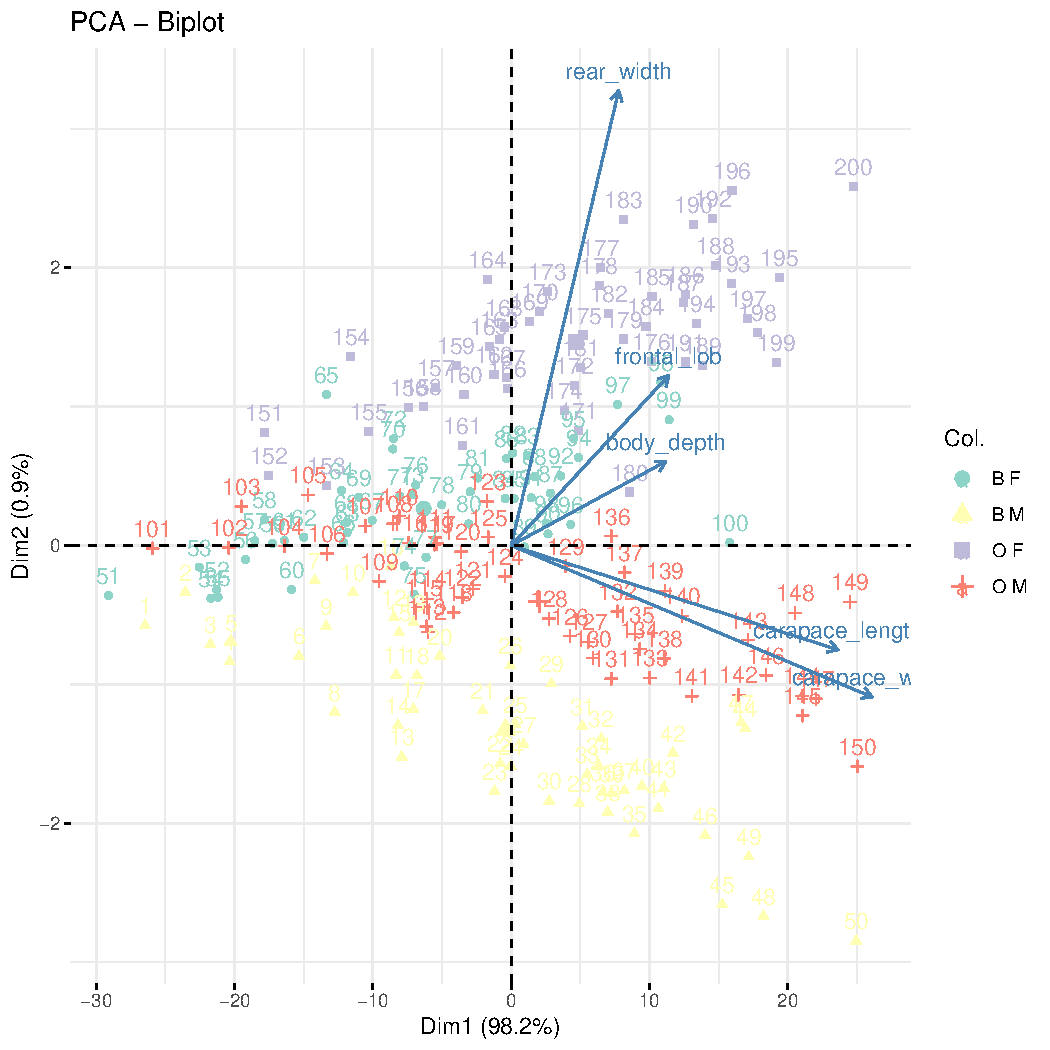
\includegraphics[width=\maxwidth]{figure/pca_crabs_untransformed-1} 

\end{knitrout}

\end{frame}

\begin{frame}[fragile,allowframebreaks]
  \frametitle{Remove size effect}
  \framesubtitle{Carried by the 1st principal component}

\paragraph{PCA is solved by SVD}
\begin{equation*}
  \mathbf{X} = \mathbf{U} \mathbf{D} \mathbf{V}^\top.
\end{equation*}

We remove the best rank-1 approximation of $\mathbf{X}$ to remove the \textit{size effect}, carried by the first axis, that is,
\begin{equation*}
  \tilde{\mathbf{X}}^{(1)} = \mathbf{U}_{\bullet 1} d_{11} \mathbf{v}_{\bullet 1}^\top.
\end{equation*}


\begin{knitrout}
\definecolor{shadecolor}{rgb}{0.969, 0.969, 0.969}\color{fgcolor}\begin{kframe}
\begin{alltt}
\hlstd{attributes} \hlkwb{<-} \hlkwd{select}\hlstd{(crabs,} \hlopt{-}\hlstd{sex,} \hlopt{-}\hlstd{species)}
\hlstd{SVD} \hlkwb{<-} \hlkwd{svd}\hlstd{(attributes)}
\hlstd{attributes_rank1} \hlkwb{<-} \hlkwd{tcrossprod}\hlstd{(SVD}\hlopt{$}\hlstd{u[,} \hlnum{1}\hlstd{]} \hlopt{*} \hlstd{SVD}\hlopt{$}\hlstd{d[}\hlnum{1}\hlstd{], SVD}\hlopt{$}\hlstd{v[,} \hlnum{1}\hlstd{])}
\hlstd{crabs_corrected} \hlkwb{<-} \hlstd{crabs}
\hlstd{crabs_corrected[,} \hlnum{3}\hlopt{:}\hlnum{7}\hlstd{]} \hlkwb{<-} \hlstd{attributes} \hlopt{-} \hlstd{attributes_rank1}
\end{alltt}
\end{kframe}
\end{knitrout}

$\rightsquigarrow$ Axis 1 explains a latent effect, here the size in the case at hand, common to all attributes.

\begin{knitrout}
\definecolor{shadecolor}{rgb}{0.969, 0.969, 0.969}\color{fgcolor}\begin{kframe}
\begin{alltt}
\hlkwd{ggpairs}\hlstd{(crabs_corrected,} \hlkwc{columns} \hlstd{=} \hlnum{3}\hlopt{:}\hlnum{7}\hlstd{,} \hlkwd{aes}\hlstd{(}\hlkwc{colour} \hlstd{= species,} \hlkwc{shape} \hlstd{= sex))}
\end{alltt}
\end{kframe}
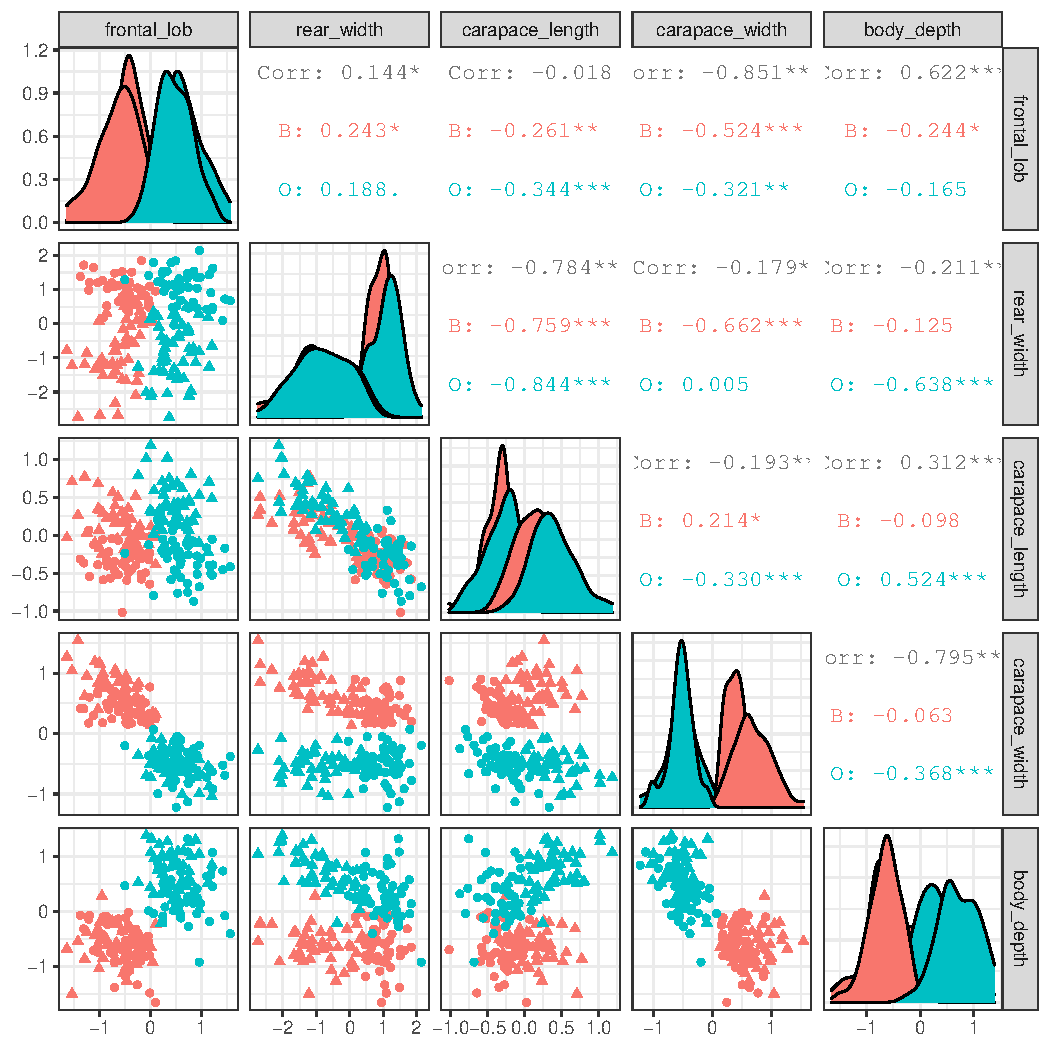
\includegraphics[width=\maxwidth]{figure/pairs_plot_corrected-1} 

\end{knitrout}

\end{frame}

\begin{frame}[fragile]
  \frametitle{PCA on corrected data}
\begin{knitrout}
\definecolor{shadecolor}{rgb}{0.969, 0.969, 0.969}\color{fgcolor}\begin{kframe}
\begin{alltt}
\hlkwd{prcomp}\hlstd{(}\hlkwd{select}\hlstd{(crabs_corrected,} \hlopt{-}\hlstd{species,} \hlopt{-}\hlstd{sex),} \hlkwc{scale.} \hlstd{=} \hlnum{TRUE}\hlstd{)} \hlopt
  \hlkwd{autoplot}\hlstd{(}\hlkwc{loadings} \hlstd{=} \hlnum{TRUE}\hlstd{,} \hlkwc{loadings.label} \hlstd{=} \hlnum{TRUE}\hlstd{,}
           \hlkwc{data} \hlstd{= crabs_corrected,} \hlkwc{colour} \hlstd{=} \hlstr{'species'}\hlstd{,} \hlkwc{shape} \hlstd{=} \hlstr{'sex'}\hlstd{)}
\end{alltt}
\end{kframe}
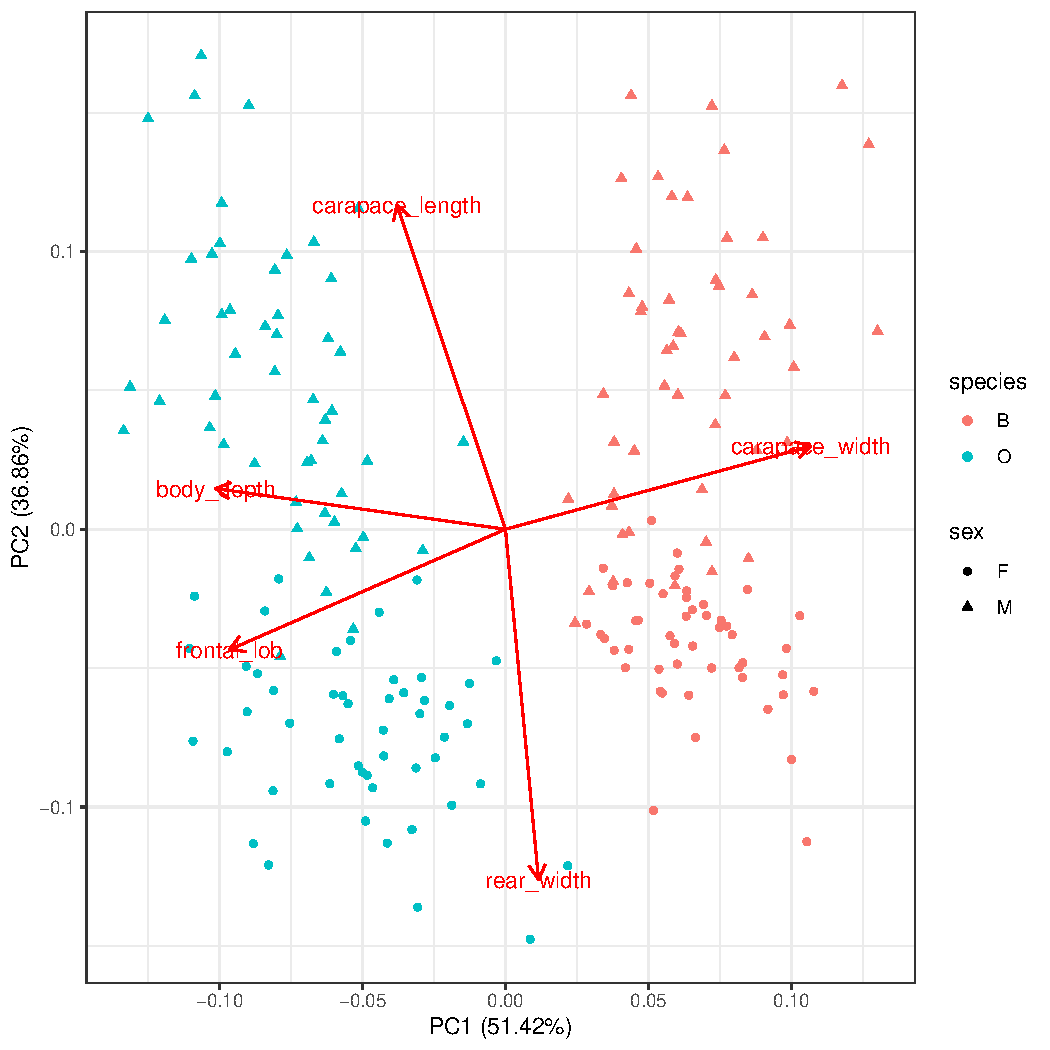
\includegraphics[width=\maxwidth]{figure/pca_crabs_corrected-1} 

\end{knitrout}
\end{frame}

\begin{frame}
  \frametitle{Questions}
  \begin{center}
    \begin{enumerate}
      \item Could we automatically identify some grouping (\alert{clustering}) between samples ?
      \item Would this clustering correspond to some known labels (sex, species)?
      \item Does it matter?
    \end{enumerate}
  \end{center}

\end{frame}

\begin{frame}[label=Clustering1]
  \frametitle{Clustering: general goals}

  \paragraph{Objective}: construct a map $f$ from $\mathcal{D}$ to $\{1,\ldots,K\}$ where $K$ is a fixed number of clusters.
    
  \vfill
    
  \paragraph{Careful! classification $\neq$ clustering}
      \begin{itemize}
      \item Classification presupposes the existence of classes
      \item Clustering labels only elements of the dataset
      \begin{itemize}
      \item[$\rightsquigarrow$] no ground truth (no given labels)
      \item[$\rightsquigarrow$] discovers a structure "natural" to the data
      \item[$\rightsquigarrow$] not necessarily related to a known classification
      \end{itemize}
      \end{itemize}
  
  \vfill

  \paragraph{Motivations}
    \begin{itemize}
    \item describe large masses of data in a simplified way,
    \item structure a set of knowledge,
    \item reveal structures, hidden causes,
    \item use of the groups in further processing, 
    \item \dots
  \end{itemize}

\end{frame}

\begin{frame}[label=Clustering2]

  \frametitle{Clustering: challenges}

    \begin{block}{Clustering quality}
      No obvious measure to define the \alert{quality} of the clusters. Ideas:
      \begin{itemize}
        \item \alert{Inner} homogeneity: samples in the same group should be similar
        \item \alert{Outer} inhomogeneity: samples in different groups should be different
      \end{itemize}
    \end{block}

    \vspace{-.25cm}

    \begin{block}{Number of clusters}
      Choice of the number of clusters $K$ often complex
      \begin{itemize}
        \item No ground truth in unsupervised learning!
        \item Several solutions might be equally good
      \end{itemize}
    \end{block}

    \vspace{-.25cm}

    \begin{block}{Two general approaches}
      \vspace{-.25cm}
      \begin{itemize}
        \item \alert{distance-based}: require a distance/dissimilarity between $\{\bx_i\}$
        \item \alert{model-based}: require assumptions on the distribution $\mathbb{P}$
      \end{itemize}
    \end{block}
    
\end{frame}

